\documentclass[fleqn]{jbook}
\usepackage{physpub}

\begin{document}

\begin{question}{$B@l96(B $BLdBj(B1}{}

% Definition of local macros

\parbox[t]{100mm}{
$B<ANL(B$m$$B$NN3;R$,H>7B(B$a$$B?<$5(B$V_{0}$$B$N0f8M7?%]%F%s%7%c%k(B
%
\[ V(r)= \left\{ \begin{array}{lc}%
         -V_{0} & (r \leq a) \\
             0  & (r>a)      \end{array} \right. \]
%
$B$NCf$r1?F0$9$k!#<!$N@_Ld$KEz$($h!#(B
%
}\parbox[t]{60mm}{\vspace*{-8mm}
\begin{center}
  \mbox{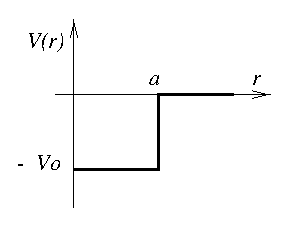
\includegraphics[clip]{1995phy1-1.eps}}
\end{center}}
%

\begin{subquestions}
\SubQuestion

  $BGHF04X?t$r6K:BI8(B$(r,\theta,\phi)$$B$G(B
  \[ \Psi (r ,\theta ,\phi )=R_{\ell}(r)Y_{\ell m}(\theta,\phi) \]
  $B$N$h$&$KI=$7$?$H$-(B$R_{\ell}(r)$$B$,=>$&J}Dx<0$r=q$1!#$?$@$7!"(B
  $B%i%W%i%7%"%s$r6K:BI8$G=q$/$H(B
%
  \[ \Laplacian = \frac{1}{r^2} \Partial{}{r}r^2 \Partial{}{r}%
                + \frac{\Operator{\Lambda}}{r^2}  \hspace{15mm}%
     \Operator{\Lambda} = \frac{1}{\sin \theta} \Partial{}{\theta} \sin\theta \Partial{}{\theta}%
                + \frac{1}{\sin^2\theta}\Partial{^2}{\phi^{2}} \]
%
  $B$N$h$&$KI=$5$l$k!#$^$?!"(B$Y_{\ell m}(\theta,\phi)$$B$O5eLLD4OB4X?t$G(B
  $B1i;;;R(B$\Operator{\Lambda}$$B$N8GM-4X?t$G$"$k!#(B
%
  \[ \Operator{\Lambda} Y_{\ell m}(\theta,\phi) = -\ell(\ell+1)Y_{\ell m}(\theta,\phi) \]
%
  \SubSubQuestion
    $V_{0}$$B$N$"$kCM$K$D$$$F$O(Bs$B>uBV(B$(\ell=0)$$B$KB+G{>uBV$,0l$D$@$1$"$j!"(B
    $B$=$NB+G{%(%M%k%.!<(B$\varepsilon$$B$O(B$V_{0}$$B$KHf$Y$F==J,>.$5$$(B
    $(0<\varepsilon \ll V_0)$$B!#(B

  \begin{subsubquestions}
  \SubSubQuestion
    $B%]%F%s%7%c%k$N?<$5(B$V_{0}$$B$r5a$a$h!#(B

  \SubSubQuestion
    $B>e$NB+G{>uBV$G$N0f8M$N30(B$(r>a)$$B$KN3;R$,B8:_$9$k3NN($r7W;;$;$h!#(B

  \end{subsubquestions}


\SubQuestion
  $B<!$KF1$8%]%F%s%7%c%k$K$h$k;6Mp$r9M$($k!#3F(B$\ell$$B$G(B$r$$B$N==J,Bg$-$$(B
  $B$H$3$m$G(B
%
  \[ R_{\ell}(r) \sim A_{\ell} \frac{ \sin{(kr- \frac{1}{2}\ell \pi + \delta_{\ell})}}{r} \]
%
  $B$GI=$5$l$F$$$k$H$-!"(B$\delta_{\ell}$ $B$r0LAj$N$:$l$H$$$&!#(B(ii)$B$HF1$8(B
  $V_{0}$$B$NCM$K$D$$$FF~<M%(%M%k%.!<$,(B$E=\frac{9V_{0}}{16}$$B$N$H$-!"(B
  s$BGH(B($\ell=0$)$B$N0LAj$N$:$l$N@5@\(B$ \tan \delta_{0}$$B$r5a$a$h!#(B

\end{subquestions}
\end{question}
\begin{answer}{$B@l96(B $BLdBj(B1}{}
 \begin{subanswers}
  \SubAnswer
Schr\"odinger$BJ}Dx<0(B
  \[
  \biggl(-\frac{\hbar^2}{2m}\Delta+V\biggr)\Psi=E\Psi
  \]
$B$G!"%i%W%i%7%"%s$r6K:BI8$GI=$7!"GHF04X?t$NF07BItJ,(B$R_l$$B$,K~$9$Y$-J}Dx<0$r(B
$BCj=P$9$k$H!"0J2<$NDL$j$H$J$k!#(B
  \begin{equation}
   \biggl(\frac{1}{r^2}\Deriver{}{r}r^2\Deriver{}{r}-\frac{l(l+1)}{r^2}\biggr)R_l
    =-\frac{2m}{\hbar^2}(E-V)R_l
  \end{equation}
  \SubAnswer
  \begin{subsubanswers}
   \SubSubAnswer
   s$B>uBV$r9M$($k$N$G(B$l=0$$B$G$"$j!"$^$?!"(B
   $\frac{1}{r^2}\Deriver{}{r}r^2\Deriver{}{r}=\frac{1}{r}\Deriver{^2}{r^2}r$
   $B$KCm0U$9$k$H!"(B$R_0$$B$,K~$9J}Dx<0$O!"(B
   \begin{align}
    \begin{array}{ll}
     \displaystyle{\Deriver{^2}{r^2}(rR_0)=
      -\frac{2m}{\hbar^2}(V_0-\varepsilon)(rR_0)}
      & \mbox{($B0f8M$NCf(B)} \\
     \displaystyle{\Deriver{^2}{r^2}(rR_0)=
      \frac{2m}{\hbar^2}\varepsilon(rR_0)}
      & \mbox{($B0f8M$N30(B)}
    \end{array}  
   \end{align}
   $B$3$l$h$j!"(B$R_0$$B$O!"A4BN$rDj?tG\$9$kG$0U@-$r=|$1$P!"(B
   \begin{equation}
    R_0=
     \begin{cases}
      \displaystyle{\frac{1}{r}
      \sin\biggl(\frac{\sqrt{2m(V_0-\varepsilon)}}{\hbar}r+\delta\biggr)}
      & (r<a) \\
      \displaystyle{
      \frac{C_1}{r}\exp\biggl(-\frac{\sqrt{2m\varepsilon}}{\hbar}r\biggr)
      +\frac{C_2}{r}\exp\biggl(\frac{\sqrt{2m\varepsilon}}{\hbar}r\biggr)}
      & (r>a)
     \end{cases}
     \eqname{eq:ro1}
   \end{equation}
   ($C_1,C_2,\delta$$B$ODj?t(B)$B$H=q$1$k!#(B

   $B$3$3$G!"GHF04X?t$N5,3J2=2DG=@-$h$j!"(B$C_2=0$$B!#$^$?86E@$G!"%]%F%s%7%c%k$,(B
   $BFC0[@-$r;}$?$J$$$3$H$h$j!"(B$\delta=0$$B$H7h$^$k!#(B

   $B;D$C$?Dj?t(B$C_1$$B$O!"(B$r=a$$B$G(B\eqhref{eq:ro1}$B$NBh(B1$B!"Bh(B2$B<0$,3j$i$+$K$D$J$,$k$h(B
   $B$&$K7hDj$5$l$k!#$3$N>r7o$O!"(B
   \begin{equation}
    \begin{cases}
     \displaystyle{
     \frac{1}{a}\sin\biggl(\frac{\sqrt{2m(V_0-\varepsilon)}}{\hbar}a\biggr)
     =\frac{C_1}{a}\exp\biggl(-\frac{\sqrt{2m\varepsilon}}{\hbar}a\biggr)} \\
     \displaystyle{
     \frac{\sqrt{2m(V_0-\epsilon)}}{\hbar}
     \cot\biggl(\frac{\sqrt{2m(V_0-\varepsilon)}}{\hbar}a\biggr)
     =-\frac{\sqrt{2m\varepsilon}}{\hbar}}
    \end{cases}
    \eqname{eq:cond1}
   \end{equation}
   $0<\varepsilon\ll V_0$$B$h$j!"(B$\varepsilon/V_0=0$$B$H$7$F$h$$!#$9$k$H!"(B
   \eqhref{eq:cond1}$BBh(B2$B<0$h$j!"(B
   \begin{align*}
    & \cot\biggl(\frac{\sqrt{2mV_0}}{\hbar}a\biggr)
    =-\sqrt{\frac{\varepsilon}{V_0}}=0 \\
    & \Longrightarrow\frac{\sqrt{2mV_0}}{\hbar}a
    =\biggl(n+\frac{1}{2}\biggr)\pi\qquad(n=0,1,2,\cdots)
   \end{align*}
   s$B>uBV$KB+G{>uBV$,$?$@0l$D$"$k$H$$$&$3$H$O!"$=$NB+G{>uBV$N8GM-4X?t$,(B
   $r<a$$B$K@a$r;}$?$J$$$3$H$r0UL#$9$k!#B($A!"(B$n=0$$B$G$"$k!#(B
   \begin{align*}
    \therefore\quad V_0 &= \biggl(\frac{\pi}{2}\biggr)^2
    \biggl(\frac{\hbar}{a}\biggr)^2\bigg/2m \\
    &= \frac{\pi^2\hbar^2}{8ma^2}
   \end{align*}
   \SubSubAnswer
   $B$3$N$H$-!"(B\eqhref{eq:cond1}$BBh(B1$B<0$O!"(B
   \[
   \sin\biggl(\frac{\pi}{2}\biggr)
   =C_1\exp\biggl(-\frac{\sqrt{2m\varepsilon}}{\hbar}a\biggr)
   \]
   $B$H$J$j!"(B
   \[
   C_1=\exp\biggl(\frac{\sqrt{2m\varepsilon}}{\hbar}a\biggr)
   \]
   $B$h$C$F!"5a$a$k3NN($O!"(B
   \begin{align*}
    \frac{\int_{a\leq r<+\infty}|\Psi|^2d^3r}
    {\int_{0\leq r<+\infty}|\Psi|^2d^3r}
    &= \frac{\int d\Omega|Y_{00}|^2\int_a^{+\infty}dr\cdot r^2|R_0|^2}
    {\int d\Omega|Y_{00}|^2\int_0^{+\infty}dr\cdot r^2|R_0|^2} \\
    &= \frac{\int_a^{+\infty}dr
    \exp\bigl(2\frac{\sqrt{2m\varepsilon}}{\hbar}a\bigr)
    \exp\bigl(-2\frac{\sqrt{2m\varepsilon}}{\hbar}r\bigr)}
    {\int_0^adr\sin^2\bigl(\frac{\pi}{2}\frac{r}{a}\bigr)
    +\int_a^{+\infty}dr
    \exp\bigl(2\frac{\sqrt{2m\varepsilon}}{\hbar}a\bigr)
    \exp\bigl(-2\frac{\sqrt{2m\varepsilon}}{\hbar}r\bigr)} \\
    &= \frac{\frac{\hbar}{2\sqrt{2m\varepsilon}}}
    {\frac{a}{2}+\frac{\hbar}{2\sqrt{2m\varepsilon}}} \\
    &= \frac{1}{1+\frac{\sqrt{2m\varepsilon}}{\hbar}a}
   \end{align*} 
  \end{subsubanswers} 
  \SubAnswer
  $(\sqrt{2mV_0}/\hbar)a=\pi/2$$B$G$"$k$3$H!"5Z$S!"0f8M$NFb$G$O(B
  $E-V=(25/16)V_0$$B!"0f8M$N30$G$O(B$E-V=(9/16)V_0$$B$G$"$k$3$H$KCm0U$9$k$H!"(B
  $R_0$$B$,=>$&J}Dx<0$O!"(B
  \begin{equation}
   \Deriver{^2}{r^2}(rR_0)=
    \begin{cases}
     \displaystyle{-\biggl(\frac{5\pi}{8}\biggr)^2\frac{1}{a^2}(rR_0)}
     & \mbox{($B0f8M$NCf(B)} \\
     \displaystyle{-\biggl(\frac{3\pi}{8}\biggr)^2\frac{1}{a^2}(rR_0)}
     & \mbox{($B0f8M$N30(B)}
    \end{cases}
  \end{equation}
  \textbf{2(i)}$B$HF1MM$N9M;!$K$h$j!"(B$R_0$$B$O!"(B
  \begin{equation}
   R_0=
    \begin{cases}
     \displaystyle{\frac{1}{r}\sin\biggl(\frac{5\pi}{8}\frac{r}{a}\biggr)}
     & (r<a) \\
     \displaystyle{\frac{C}{r}\sin\biggl(\frac{3\pi}{8}\frac{r}{a}
     +\delta_0\biggr)} & (r>a)
    \end{cases}
  \end{equation}
  ($C$$B$ODj?t(B)$B$H=q$1$k!#$3$l$i$,!"(B$r=a$$B$G3j$i$+$K$D$J$,$k$3$H$h$j!"(B$rR_0$$B$N(B
  $BBP?tHyJ,$,(B$r=a$$B$G0lCW$9$k!#$h$C$F!"(B
  \begin{align}
   & \frac{5\pi}{8}\cot\biggl(\frac{5\pi}{8}\biggr) 
   = \frac{3\pi}{8}\cot\biggl(\frac{3\pi}{8}+\delta_0\biggr)\notag\\
   & \Longleftrightarrow
   \tan\biggl(\frac{3\pi}{8}+\delta_0\biggr)
   =\frac{3}{5}\tan\biggl(\frac{5\pi}{8}\biggr) \notag\\
   & \mspace{-18.0mu}\mbox{$B2CK!DjM}$rMQ$$$F!":8JU$N(B$\tan$$B$rJ,2r$7$F@0M}(B
   $B$9$k$H(B} \notag\\
   & \Longleftrightarrow
   \tan\delta_0=\frac{\frac{3}{5}\tan\frac{5\pi}{8}-\tan\frac{3\pi}{8}}
   {1+\frac{3}{5}\tan\frac{3\pi}{8}\tan\frac{5\pi}{8}}\eqname{eq:delta0}
  \end{align}
  $B0lJ}(B
  \[
   \tan\frac{5\pi}{8}=\tan\biggl(\pi-\frac{3\pi}{8}\biggr)=-\tan\frac{3\pi}{8}
  \]
  $B5Z$S!"(B$\tan$$B$N2CK!DjM}(B
  \begin{align*}
   1 &= \tan\biggl(\frac{5\pi}{8}-\frac{3\pi}{8}\biggr) \\
   &= \frac{\tan\frac{5\pi}{8}-\tan\frac{3\pi}{8}}
   {1+\tan\frac{5\pi}{8}\tan\frac{3\pi}{8}}
  \end{align*}
  $B$h$j!"(B
  \[
  \tan\frac{3\pi}{8}=1+\sqrt{2},\qquad\tan\frac{5\pi}{8}=-1-\sqrt{2}
  \]
  $B$J$N$G!"$3$l$r(B\eqhref{eq:delta0}$B$KBeF~$7$F7W;;$9$k$H!"(B
  \[
   \tan\delta_0=\frac{8+2\sqrt{2}}{7}
  \]
  $B$H$J$k!#(B
 \end{subanswers}
\end{answer}

\end{document}
